
\section{Baurecht und Haftung}
\label{section:antennen_baurecht_haftung}
\begin{frame}%STARTCONTENT

\begin{columns}
    \begin{column}{0.48\textwidth}
    
\begin{figure}
    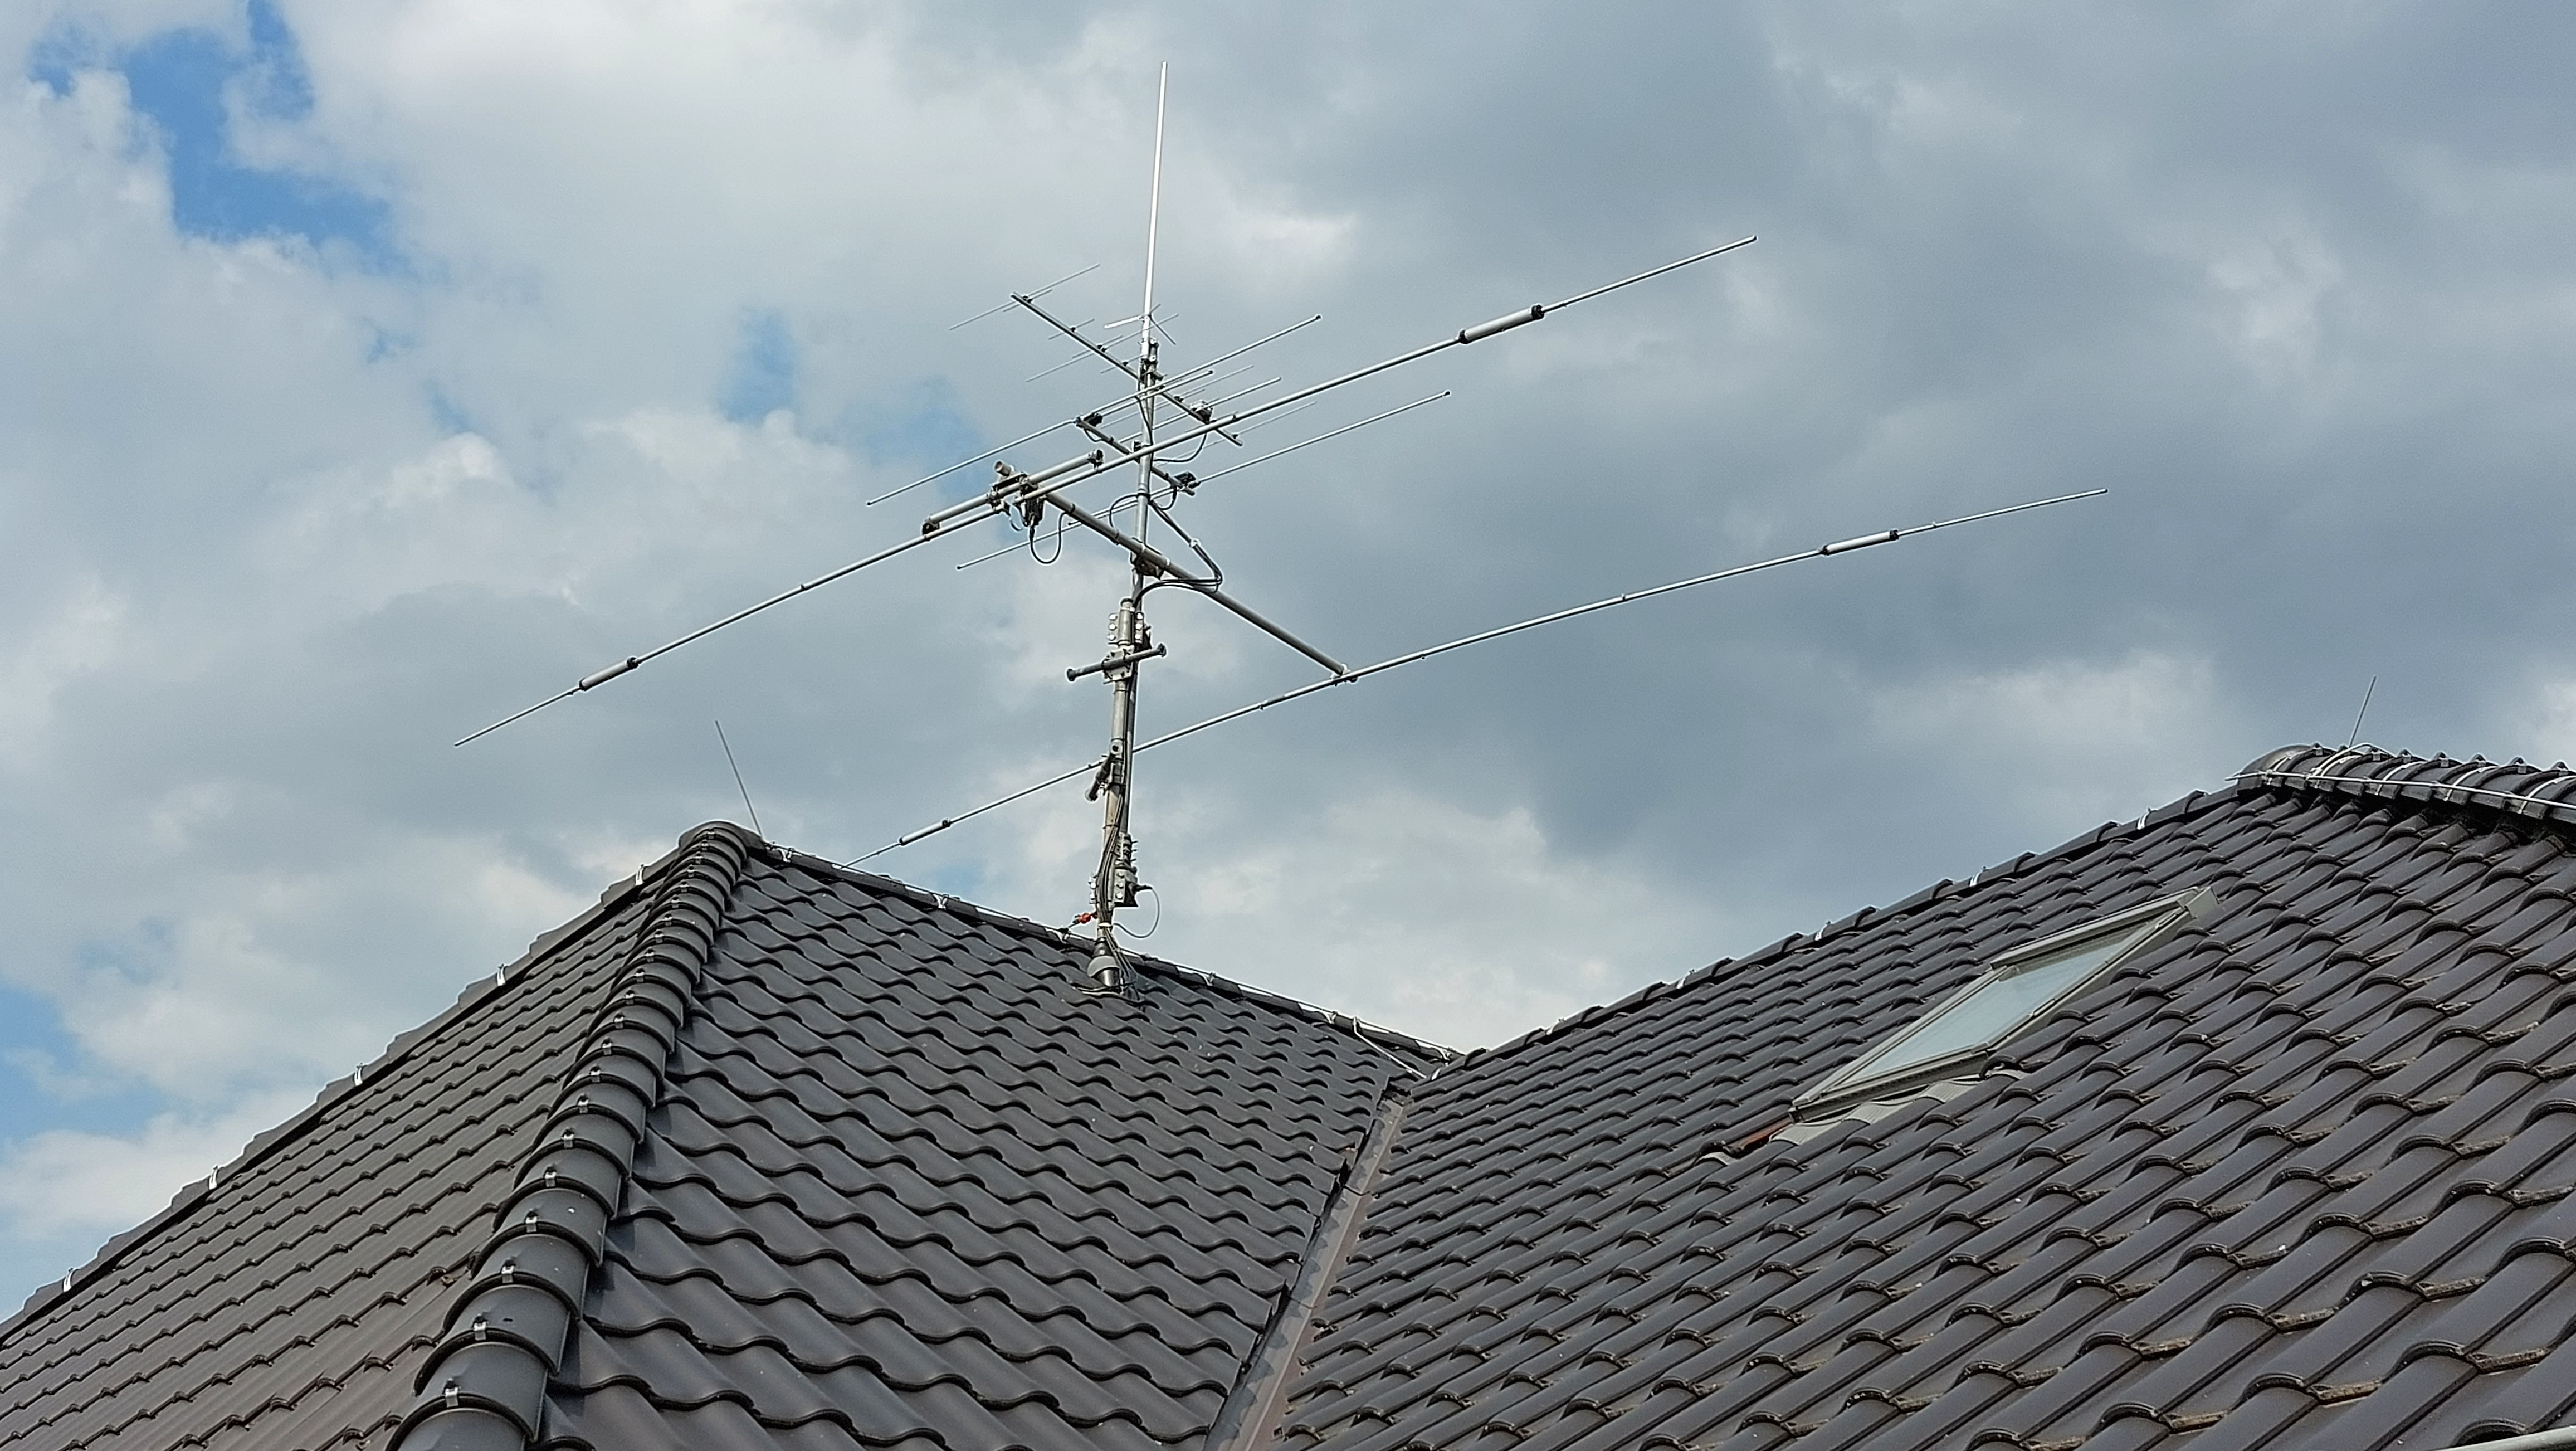
\includegraphics[width=0.85\textwidth]{foto/83}
    \caption{\scriptsize Antennenanlage für KW, VHF und UHF auf einem Hausdach}
    \label{n_antennen_hausdach}
\end{figure}

    \end{column}
   \begin{column}{0.48\textwidth}
       \begin{itemize}
  \item Baurechtliche Bestimmungen des Bundeslandes
  \item Höhe, Abstände zu Nachbargrundstücken, Windlast, etc.
  \item Es haftet der Eigentümer oder Betreiber der Antennenanlage
  \end{itemize}

   \end{column}
\end{columns}

\end{frame}

\begin{frame}
\only<1>{
\begin{QQuestion}{VE602}{Nach welchen Bauvorschriften müssen Außenantennenanlagen errichtet werden?}{Für private Amateurfunkanlagen sind keine besonderen Vorschriften zu beachten.}
{Es gelten die Bestimmungen des Amateurfunkgesetzes (AFuG).}
{Es sind nur die Empfehlungen der Amateurfunkverbände zu beachten.}
{Es gelten die baurechtlichen Bestimmungen des jeweiligen Bundeslandes.}
\end{QQuestion}

}
\only<2>{
\begin{QQuestion}{VE602}{Nach welchen Bauvorschriften müssen Außenantennenanlagen errichtet werden?}{Für private Amateurfunkanlagen sind keine besonderen Vorschriften zu beachten.}
{Es gelten die Bestimmungen des Amateurfunkgesetzes (AFuG).}
{Es sind nur die Empfehlungen der Amateurfunkverbände zu beachten.}
{\textbf{\textcolor{DARCgreen}{Es gelten die baurechtlichen Bestimmungen des jeweiligen Bundeslandes.}}}
\end{QQuestion}

}
\end{frame}

\begin{frame}
\only<1>{
\begin{QQuestion}{VE707}{Wer haftet für Schäden gegenüber Dritten, die durch die Antennenanlage einer Amateurfunkstelle entstehen können?}{Die Amateurfunkvereinigung, wenn der Betreiber der Amateurfunkstelle Mitglied einer solchen Vereinigung ist}
{Der Eigentümer oder Betreiber der Antennenanlage}
{Die Bundesnetzagentur, da in den monatlichen Beiträgen auch ein Anteil für eine Gruppenversicherung für Antennenanlagen von Funkamateuren enthalten ist.}
{Der Grundstückseigentümer, er hat eine Antennenhaftpflichtversicherung abzuschließen, selbst wenn er nicht Betreiber der Amateurfunkstelle ist.}
\end{QQuestion}

}
\only<2>{
\begin{QQuestion}{VE707}{Wer haftet für Schäden gegenüber Dritten, die durch die Antennenanlage einer Amateurfunkstelle entstehen können?}{Die Amateurfunkvereinigung, wenn der Betreiber der Amateurfunkstelle Mitglied einer solchen Vereinigung ist}
{\textbf{\textcolor{DARCgreen}{Der Eigentümer oder Betreiber der Antennenanlage}}}
{Die Bundesnetzagentur, da in den monatlichen Beiträgen auch ein Anteil für eine Gruppenversicherung für Antennenanlagen von Funkamateuren enthalten ist.}
{Der Grundstückseigentümer, er hat eine Antennenhaftpflichtversicherung abzuschließen, selbst wenn er nicht Betreiber der Amateurfunkstelle ist.}
\end{QQuestion}

}
\end{frame}%ENDCONTENT
